\documentclass[../structural_economics_book.tex]{subfiles}
\begin{document}
\ifSubfilesClassLoaded{\setcounter{chapter}{22}}{}
\chapter{Tracking Structural Change Over Time}\label{ch:23}
\chaptersubtitle{The Moving Heatmap}
\begin{quote}
\textit{``El cambio estructural no es un evento sino un proceso: una secuencia de transformaciones en las relaciones entre los componentes del sistema econ\'{o}mico.''}\\[0.3em]
\textnormal{[``Structural change is not an event but a process: a sequence of transformations in the relations between the components of the economic system.'']}\\
\hfill --- CEPAL, \textit{Cambio estructural para la igualdad: una visi\'{o}n integrada del desarrollo} (2012)
% TODO-VERIFY: this sentence was not located verbatim in CEPAL (2012), LC/G.2524(SES.34/3); check the Spanish edition and give a page, or present it as a paraphrase.
\end{quote}
\nocite{cepal2012cambio}

\vspace{1em}

Chapters~20--22 showed how to measure $W^P$, $W^I$, and $W^U$ at a single point in time. This chapter adds the time dimension: how to track $W_t$ across years, detect structural breaks, measure the speed of change, and distinguish structural change from cyclical fluctuation.

The central object is the \textbf{structural trajectory}: the time series of $\Gamma_t$, $\sigma_{B,t}$, $G(\boldsymbol{\pi}_t)$ and $N_{\text{eff},t}$ computed from a sequence of SAMs or equivalent data. The trajectory tells you whether the economy is integrating or fragmenting, at what speed, and whether specific events (a nationalization, a trade reform, a crisis) produced detectable structural effects.

Chapter~17 previewed Bolivia's trajectory. This chapter develops the methods and applies them to data. Two conventions are in force throughout (Chapter~1, Section~\ref{ch01:sec:conventions}): $\Gamma$ measures \emph{integration} (mixing speed) only, and the concentration of power is measured by $\Neff$, $\Var(\boldsymbol{\pi})$ or $G(\boldsymbol{\pi})$, never by $\Gamma$ (Proposition~\ref{ch06:prop:gap-power-independent}).

The production-network trajectories are sourced. For Bolivia they come from INE's symmetric input--output matrices (base 1990, 1988--2014) and supply-use tables (base 2017, 2017--2024) \citep{ine2026sut}. The two bases differ in classification and national-accounts vintage, so they are kept as two separate series and no change is ever computed across the break. For Korea and the comparators they come from the domestic blocks of the OECD Inter-Country Input-Output tables, 2021 edition for 1995--2014 and 2023 edition for 2011--2020 \citep{oecd2021icio,oecd2023icio}. Complexity is the Growth Lab's ECI \citep{growthlab2026atlas}. Throughout, $\Gamma$ is that of the 12-sector domestic input-share matrix $W^P = D^{-1}A$ with the diagonal kept: the book's 12-sector classification for Bolivia's own series, and an ISIC-based 12-sector classification for comparisons across countries (Bolivia 2019: $\Gamma = 0.467$ and $0.475$ respectively). $\Gamma$ depends on aggregation and normalization. For Bolivia in 2019 it ranges from 0.33 to 0.69 across input and sales shares, with and without the diagonal, at 12 and 39 sectors, so only like-for-like comparisons are meaningful. Between-block inequality $\sigma_B$ and information concentration $\Neff(W^I)$ need household and audience microdata that were not available: their values remain \illustrative. Every sourced number is read from \path{data/processed} and checked by \texttt{code/ch23.py}.

The data do not tell the story usually told about Bolivia, and the chapter follows the data. Bolivia's $\Gamma$ is not low by comparison; it drifted \emph{down}, and so did Korea's. What separates the two economies is complexity, not aggregate integration.


%% =====================================================================
\section{The Time-Varying Weight Matrix}
\label{ch23:sec:time_varying}
%% =====================================================================

\subsection{Construction}

\begin{definition}[Time-Indexed Weight Matrix]\label{ch23:def:Wt}
For each year $t$, construct $W_t$ from the available data:
\begin{enumerate}
\item $W^P_t$: from the I-O table (if available for year $t$) or interpolated from benchmark I-O tables using annual National Accounts.
\item $W^I_t$: from media audience data (annual surveys) or digital trace data (continuous).
\item $W^U_t$: from household surveys (typically annual or biennial).
\end{enumerate}
The structural indicators are computed annually: $\Gamma_t = \Gamma(W_t)$, $\boldsymbol{\pi}_t = \boldsymbol{\pi}(W_t)$, etc.
\end{definition}

\begin{definition}[Interpolation of $W^P$ Between Benchmark I-O Tables]\label{ch23:prop:interpolation}
Most countries produce I-O tables only every 5--10 years. Between benchmarks, $W^P_t$ can be approximated by:
\begin{equation}\label{ch23:eq:interpolation}
W^P_t \approx W^P_{\tau_0} + \frac{t - \tau_0}{\tau_1 - \tau_0}(W^P_{\tau_1} - W^P_{\tau_0}),
\end{equation}
where $\tau_0$ and $\tau_1$ are the benchmark years. Because the right-hand side is a convex combination of two row-stochastic matrices, it is itself row-stochastic. Alternatively, use the RAS method on the intermediate-transactions matrix $Z_{\tau_0}$ (not on $W^P$): given the year-$t$ intermediate sales $\mathbf{u}_t$ (row totals of $Z_t$) and intermediate purchases $\mathbf{v}_t$ (column totals) from annual National Accounts, with $\ones'\mathbf{u}_t = \ones'\mathbf{v}_t$, rescale $Z_{\tau_0}$ biproportionally to these margins and then row-normalize:
\begin{equation}\label{ch23:eq:RAS}
Z_t = \text{RAS}(Z_{\tau_0}; \mathbf{u}_t, \mathbf{v}_t), \qquad W^P_t = D_t^{-1}Z_t, \quad D_t = \operatorname{diag}(Z_t\ones).
\end{equation}
RAS preserves the zero pattern (hence the block structure) of $Z_{\tau_0}$ while adjusting for changes in sectoral composition. A solution exists only if the margins are consistent and compatible with the zero pattern (Appendix~\ref{ch23:app:RAS}).
\end{definition}


\subsection{The Structural Trajectory}

\begin{definition}[Structural Trajectory]\label{ch23:def:trajectory}
The \textbf{structural trajectory} of an economy is the time series:
\begin{equation}\label{ch23:eq:trajectory}
\mathcal{T} = \{(\Gamma_t, \sigma_{B,t}, G(\boldsymbol{\pi}_t), N_{\text{eff},t}, \text{ECI}_t) : t = t_0, \ldots, T\}.
\end{equation}
The trajectory is plotted in the five-dimensional structural health space (Chapter~17). Projection onto the $(\Gamma_t, \sigma_{B,t})$ plane gives a useful two-dimensional visualization: integration on one axis, between-block inequality on the other. Power concentration ($G(\boldsymbol{\pi}_t)$, $N_{\text{eff},t}$) is a separate coordinate and must be read separately.
\end{definition}


\subsection{Products of Time-Varying Matrices}
\label{ch23:sec:products}

The per-period indicators $\Gamma(W_t)$ and $\boldsymbol{\pi}(W_t)$ describe a frozen snapshot. The economy, however, is driven by the \emph{sequence}. In the information reading, beliefs evolve as $\bb_{t+1} = W_t\bb_t$, so after several periods
\begin{equation}\label{ch23:eq:backward_product}
\bb_t = P_{t,s}\,\bb_s, \qquad P_{t,s} := W_{t-1}W_{t-2}\cdots W_s \quad (t > s),
\end{equation}
a \emph{backward product} of row-stochastic matrices. What matters for integration over a decade is the mixing of $P_{t,s}$, not of each factor.

\begin{remark}[Per-period $\Gamma$ does not control the product]\label{ch23:rem:product_counterexample}
$|\lambda_2|$ is not submultiplicative. Take
\[
X = \begin{pmatrix} 1 & 0 & 0\\ 0 & 0 & 1\\ 0.85 & 0 & 0.15 \end{pmatrix}, \qquad
Y = \begin{pmatrix} 0 & 0.95 & 0.05\\ 0 & 1 & 0\\ 1 & 0 & 0 \end{pmatrix}.
\]
Then $\Gamma(X) = 0.850$ and $\Gamma(Y) = 0.776$, but $\Gamma(XY) = 0.042$. A trajectory that alternates $X$ and $Y$ shows a ``healthy'' per-period $\Gamma_t$ while the realized two-period dynamics barely mix (realized gap per period $1 - |\lambda_2(XY)|^{1/2} = 0.021$). Numbers from \texttt{code/ch23.py}.
\end{remark}

The right instrument is the \textbf{Dobrushin ergodicity coefficient}
\begin{equation}\label{ch23:eq:dobrushin}
\tau_1(W) := \tfrac{1}{2}\max_{i,j}\sum_k |W_{ik} - W_{jk}| \;\in [0,1],
\end{equation}
the largest total-variation distance between two rows. $\tau_1(W) < 1$ iff every two rows share some column with positive weight (``$W$ is scrambling'').

\begin{proposition}[Properties of $\tau_1$]\label{ch23:prop:dobrushin}
For row-stochastic $A$, $B$: (i) $\tau_1(AB) \le \tau_1(A)\,\tau_1(B)$; (ii) every eigenvalue $\lambda \neq 1$ of $A$ satisfies $|\lambda| \le \tau_1(A)$, so $\Gamma(A) \ge 1 - \tau_1(A)$.
\end{proposition}
\begin{proof}
\emph{Step 1: $\tau_1$ is an operator norm.} Let $\mathcal{Z} := \{\boldsymbol{\delta} \in \R^N : \boldsymbol{\delta}'\ones = 0\}$. We show $\|\boldsymbol{\delta}'A\|_1 \le \tau_1(A)\|\boldsymbol{\delta}\|_1$ for all $\boldsymbol{\delta} \in \mathcal{Z}$, with equality for $\boldsymbol{\delta} = \mathbf{e}_i - \mathbf{e}_j$ at the maximizing pair $(i,j)$ in \eqref{ch23:eq:dobrushin}. If $\boldsymbol{\delta} \in \mathcal{Z}\setminus\{0\}$, write $\boldsymbol{\delta} = c(\mathbf{p} - \mathbf{q})$ with $c = \|\boldsymbol{\delta}\|_1/2$ and $\mathbf{p} = \boldsymbol{\delta}^+/c$, $\mathbf{q} = \boldsymbol{\delta}^-/c$ probability vectors (positive and negative parts have equal mass because $\boldsymbol{\delta}'\ones = 0$). Then $\mathbf{p}'A - \mathbf{q}'A = \sum_{i,j}p_iq_j(A_{i\cdot} - A_{j\cdot})$, so $\|\boldsymbol{\delta}'A\|_1 \le c\max_{i,j}\|A_{i\cdot} - A_{j\cdot}\|_1 = 2c\,\tau_1(A) = \tau_1(A)\|\boldsymbol{\delta}\|_1$. Since $A\ones = \ones$, $\boldsymbol{\delta}'A\ones = 0$: $\mathcal{Z}$ is invariant under $\boldsymbol{\delta}' \mapsto \boldsymbol{\delta}'A$.

\emph{(i)} For $\boldsymbol{\delta} \in \mathcal{Z}$, $\boldsymbol{\delta}'A \in \mathcal{Z}$, so $\|\boldsymbol{\delta}'AB\|_1 \le \tau_1(B)\|\boldsymbol{\delta}'A\|_1 \le \tau_1(B)\tau_1(A)\|\boldsymbol{\delta}\|_1$. Taking $\boldsymbol{\delta} = \mathbf{e}_i - \mathbf{e}_j$ ($\|\boldsymbol{\delta}\|_1 = 2$) gives $\tfrac12\|(AB)_{i\cdot} - (AB)_{j\cdot}\|_1 \le \tau_1(A)\tau_1(B)$ for every pair $(i,j)$.

\emph{(ii)} Let $\mathbf{u} \in \mathbb{C}^N\setminus\{0\}$ satisfy $\mathbf{u}'A = \lambda\mathbf{u}'$ with $\lambda \ne 1$. Then $\lambda\,\mathbf{u}'\ones = \mathbf{u}'A\ones = \mathbf{u}'\ones$, so $\mathbf{u}'\ones = 0$. Write $\mathbf{u} = \mathbf{x} + i\mathbf{y}$ with $\mathbf{x}, \mathbf{y} \in \mathcal{Z}$ real. Since $A$ is real, $\mathbf{x}'A^n = \operatorname{Re}(\lambda^n\mathbf{u}')$ and $\mathbf{y}'A^n = \operatorname{Im}(\lambda^n\mathbf{u}')$, and by (i) applied $n$ times, $\|\mathbf{x}'A^n\|_1 \le \tau_1(A)^n\|\mathbf{x}\|_1$, and likewise for $\mathbf{y}$. Hence
\[
|\lambda|^n\|\mathbf{u}\|_1 = \|\lambda^n\mathbf{u}'\|_1 \le \|\mathbf{x}'A^n\|_1 + \|\mathbf{y}'A^n\|_1 \le \tau_1(A)^n(\|\mathbf{x}\|_1 + \|\mathbf{y}\|_1) \le 2\,\tau_1(A)^n\|\mathbf{u}\|_1,
\]
so $|\lambda| \le 2^{1/n}\tau_1(A)$ for every $n$; let $n \to \infty$. (For real $\lambda$ the case $n = 1$ already suffices.) For the bound on $\Gamma$: if $1$ is a simple eigenvalue, $|\lambda_2| \le \tau_1(A)$ by what was just shown. If $1$ is a repeated eigenvalue then $\Gamma(A) = 0$; since $A^n$ is bounded, $1$ is semisimple, so there are two independent left eigenvectors for $1$, and a combination $\mathbf{u} \in \mathcal{Z}\setminus\{0\}$ of them satisfies $\mathbf{u}'A = \mathbf{u}'$; Step~1 then forces $\tau_1(A) \ge 1$, i.e.\ $\tau_1(A) = 1$, and the bound holds with equality. These are the standard properties of the coefficient of ergodicity \citep[Sect.~4.3]{seneta2006nonnegative}; \texttt{code/ch23.py} checks (i), (ii) and the norm identity of Step~1 on random matrices.
\end{proof}

In the counterexample, $\tau_1(X) = \tau_1(Y) = \tau_1(XY) = 1$: neither matrix is scrambling, which flags the problem that $\Gamma_t$ hides.

\begin{definition}[Weak and Strong Ergodicity]\label{ch23:def:ergodicity}
The sequence $(W_t)$ is \textbf{weakly ergodic} if $\tau_1(P_{t,s}) \to 0$ as $t \to \infty$ for every $s$: the rows of the product become equal, so the system forgets its initial condition and reaches consensus. It is \textbf{strongly ergodic} if, in addition, $P_{t,s} \to \ones\mathbf{v}_s'$ for some probability vector $\mathbf{v}_s$.
\end{definition}

\begin{proposition}[A Sufficient Condition for Weak Ergodicity]\label{ch23:prop:hajnal}
If $\sum_{t}\bigl(1 - \tau_1(W_t)\bigr) = \infty$, then $(W_t)$ is weakly ergodic.
\end{proposition}
\begin{proof}
Fix $s$. By Proposition~\ref{ch23:prop:dobrushin}(i), applied $t-s-1$ times, $\tau_1(P_{t,s}) \le \prod_{r=s}^{t-1}\tau_1(W_r) \le \exp\bigl(-\sum_{r=s}^{t-1}(1-\tau_1(W_r))\bigr)$, using $x \le e^{-(1-x)}$ for $x \in [0,1]$ (convexity of the exponential: $e^{z} \ge 1 + z$ with $z = x - 1$). Removing the finitely many terms $r < s$ from a divergent series of nonnegative terms leaves it divergent, so the exponent tends to $-\infty$ and $\tau_1(P_{t,s}) \to 0$. This is Hajnal's condition \citep{hajnal1958weak}; see \citet[Sect.~4.4]{seneta2006nonnegative}.
% TODO-VERIFY: section numbers 4.3 (coefficients of ergodicity) and 4.4 (sufficient conditions for weak ergodicity) in Seneta (2006, Springer revised printing).
\end{proof}

For backward products such as \eqref{ch23:eq:backward_product}, weak and strong ergodicity coincide \citep[ch.~4]{chatterjee1977towards,seneta2006nonnegative}, and the limit vector has a direct power interpretation. An \textbf{absolute probability sequence} is a sequence of probability vectors $(\boldsymbol{\pi}_t)$ with $\boldsymbol{\pi}_{t+1}'W_t = \boldsymbol{\pi}_t'$ \citep{kolmogorov1936theorie,touri2014product}. Such a sequence always exists, and it makes $\boldsymbol{\pi}_t'\bb_t$ invariant, since $\boldsymbol{\pi}_{t+1}'\bb_{t+1} = \boldsymbol{\pi}_{t+1}'W_t\bb_t = \boldsymbol{\pi}_t'\bb_t$. Under weak ergodicity the eventual consensus is therefore $\boldsymbol{\pi}_s'\bb_s$: \emph{$\boldsymbol{\pi}_s$, not $\boldsymbol{\pi}(W_s)$, is the time-varying vector of epistemic power.} When $W_t$ changes slowly, $\boldsymbol{\pi}_t \approx \boldsymbol{\pi}(W_t)$, with an error controlled by the perturbation lemma (Lemma~\ref{ch06:lem:perturbation}).

\begin{keyinsight}
Report three integration diagnostics, not one: the per-period gap $\Gamma(W_t)$; the Dobrushin coefficient $\tau_1(W_t)$, which composes over time; and the \emph{realized-product gap} over a window of $k$ years, $\Gamma^{(k)}_t := 1 - |\lambda_2(W_{t+k-1}\cdots W_t)|^{1/k}$. When they disagree, the realized-product gap is the one that describes what actually happened.
\end{keyinsight}


%% =====================================================================
\section{Detecting Structural Breaks}
\label{ch23:sec:breaks}
%% =====================================================================

\begin{definition}[Structural Break]\label{ch23:def:break}
A \textbf{structural break} at time $t^*$ is a discontinuity in the trajectory $\mathcal{T}$: a change in $\Gamma$, $\sigma_B$, or $\boldsymbol{\pi}$ that is larger than can be explained by normal cyclical variation. Formally, a break at $t^*$ if:
\begin{equation}\label{ch23:eq:break}
|\Gamma_{t^*+1} - \Gamma_{t^*}| > k \cdot \hat{\sigma}_{\Delta\Gamma},
\end{equation}
where $\hat{\sigma}_{\Delta\Gamma}$ is the standard deviation of year-to-year changes in $\Gamma$ during a stable period, and $k$ is the detection threshold (typically $k = 2$ or $k = 3$).
\end{definition}

\begin{remark}[Breaks in $\boldsymbol{\pi}$ need error bands]\label{ch23:rem:conditioning}
The Perron vector is badly conditioned exactly when $\Gamma$ is small. By the perturbation lemma (Lemma~\ref{ch06:lem:perturbation}), $d\boldsymbol{\pi}' = \boldsymbol{\pi}'E\,Z$ with $Z = (I - W + \ones\boldsymbol{\pi}')^{-1}$, and $Z$ is large when $\lambda_2$ is close to $+1$. In the two-block matrix of \texttt{code/ch23.py}, moving weight $\delta$ from a within-block to a cross-block entry of one row changes block~1's power at rate $-1.28$ when $\Gamma = 0.13$, against $-0.37$ when $\Gamma = 0.45$: about 3.5 times more sensitive. In a weakly coupled dual economy with $\Gamma = 0.13$, measurement error in $W_t$ is strongly amplified in $\boldsymbol{\pi}_t$. Bolivia's measured $\Gamma$ (0.47--0.57 at 12 sectors) is in the second regime, so amplification through $Z$ is moderate there. The larger source of spurious breaks in Bolivia's series is construction: the change of base, years without a published make matrix, and inconsistencies in the published tables (Example~\ref{ch23:ex:epochs}). Before declaring a break in $\Gamma$ or $\boldsymbol{\pi}$, bootstrap the underlying data (resample survey households, perturb I-O cells within their revision ranges), recompute $\Gamma_t$ and $\boldsymbol{\pi}_t$, and require the change to exceed the bootstrap band as well as $k\hat{\sigma}$.
\end{remark}

\begin{definition}[Types of Structural Breaks]\label{ch23:prop:break_types}
Three types of structural breaks correspond to three types of $\Delta W$:
\begin{enumerate}
\item \textbf{Edge creation break}: new edges appear (a trade agreement, infrastructure project, market opening). New \emph{cross-block} edges in a weakly coupled structure raise $\Gamma$ (they raise the conductance, which bounds $\Gamma$ from below for reversible $W$); new \emph{within-block} edges can lower it. Example: South Korea's export push (1960s).
\item \textbf{Edge destruction break}: edges are severed (a crisis, sanctions, nationalization). $\Gamma$ may decrease or increase depending on which edges are destroyed (cross-block destruction lowers $\Gamma$; within-block destruction may increase it). Example: Soviet collapse (1991).
\item \textbf{Reweighting break}: existing edge weights shift (a terms-of-trade shock, a technological change that alters input shares). $\Gamma$ changes smoothly rather than discretely. Example: the commodity supercycle (2003--2014).
\end{enumerate}
Whether a break is \emph{structural} or \emph{cyclical} is a separate question (Definition~\ref{ch23:def:decomposition}): any of the three types is structural if it persists and cyclical if it reverses.
\end{definition}


%% =====================================================================
\section{Bolivia's Structural Trajectory, 1988--2024}
\label{ch23:sec:bolivia}
%% =====================================================================

\begin{example}[Bolivia: Five Structural Epochs]\label{ch23:ex:epochs}
INE publishes symmetric input--output matrices for every year 1988--2009 and 2011--2014 on base 1990, and supply-use tables for 2017--2024 on base 2017. There are no tables for 2010, 2015 or 2016. $\Gamma$ below is that of the 12-sector domestic input-share matrix; complexity is the ECI (HS92, available from 1995). Household microdata were not available, so the $\sigma_B$ values are \illustrative.

\textbf{Epoch 1: Structural Adjustment (1985--1993).} The NEP (New Economic Policy) liberalized trade, closed state mines, and privatized public enterprises. Expected effect: edge destruction (state mining edges severed) and edge creation (new private-sector trade edges).

Trajectory: the tables begin in 1988, after the 1985--87 mine closures, so the shock itself is not observed. From 1988 to 1993, $\Gamma$ was flat (0.563 to 0.573), and the hydrocarbons sector's Perron weight was small (0.025 in 1988). Illustratively, $\sigma_B$ rose from $\approx 0.65$ to $\approx 0.68$ as mining workers were expelled into the informal sector.

\textbf{Epoch 2: Capitalization and Gas Discovery (1994--2005).} The ``capitalization'' of state enterprises brought FDI into gas, telecoms, and transport. Gas production began at Sab\'{a}lo and San Alberto fields.

Trajectory: $\Gamma$ \emph{fell}, from 0.567 in 1994 to 0.502 in 2005, most of it in a level shift around 1999--2000 (see the break test below). The gas sector connected primarily to the rest of the world: the share of its output exported rose from 22\% in 2000 to 69\% in 2006. Its Perron weight in the domestic $W^P$ rose from 0.022 (1994) to 0.074 (2005), still below the uniform share $1/N$. Bolivia's weight in the global trade network rose from 0.00018 (1995) to 0.00047 (2006) (Chapter~16). ECI fell by 0.24 (1995 to 2005). Illustratively, $\sigma_B$ fell from 0.68 to 0.63 as gas revenue created government jobs, moving some workers from the informal to the formal block.

\textbf{Epoch 3: Gas Nationalization (2006--2009).} The Hydrocarbons Law 3058 (2005) had already raised the state's take to 50\% (18\% royalties plus the 32\% direct hydrocarbons tax, IDH). Supreme Decree 28701 (May 2006) imposed a transitional 82\% take on the two largest fields (San Alberto and Sab\'{a}lo) while all contracts were renegotiated.

Trajectory: no detectable structural break in $\Gamma$: 0.518 in 2006 and 0.504 in 2009. The nationalization changed the \textit{distribution} of existing flows (gas $\to$ MNC profit repatriation shifted to gas $\to$ treasury), a persistent reweighting of ownership and fiscal flows that the inter-industry $W^P$ does not record. It did not create new domestic production edges: hydrocarbons bought 0.381 of domestic intermediate inputs per unit of output in 2006, and their Perron weight moved within 0.064--0.087. The government's and foreign owners' shares of the circular flow shifted, but measuring that needs a SAM (Chapter~20), not $W^P$. ECI fell by 0.14. Illustratively, $\sigma_B$ fell modestly (0.63 to 0.61) as fiscal transfers reached poor households.

\textbf{Epoch 4: Redistribution Without Structural Change (2010--2019).} A decade of high gas revenue, large fiscal transfers (Bono Juancito Pinto, Renta Dignidad, subsidies), and poverty reduction.

Trajectory: no single base spans the decade. On base 1990, $\Gamma$ was 0.478 in 2011 and 0.484 in 2013; on base 2017, 0.506 in 2017 and 0.467 in 2019. ECI stayed at its low level: $-1.28$ in 2010, $-1.30$ in 2019, with Bolivia's rank falling from 127th to 131st. Illustratively, $\sigma_B$ held at 0.61--0.62 and $\Neff(W^I)$ rose slowly ($3.0 \to 3.4$, driven by social media; 3.4 is the end-of-period value on Chapter~17's four media ecosystems, Example~\ref{ch17:ex:bolivia_neff}). Meanwhile the distributional record was remarkable. The Gini of per-capita household income fell from 0.600 (2005) to 0.426 (2019), and extreme poverty from 38.2\% (2005) to 15.2\% (2018). Ten years of redistribution produced no rise in $\Gamma$ and no gain in complexity, and large equity gains anyway.

\textbf{Epoch 5: Crisis and Stagnation (2019--present).} Political crisis (2019), pandemic (2020--2021), declining gas reserves.

Trajectory: on base 2017, $\Gamma$ fell from 0.467 (2019) to 0.381 (2023) and was 0.419 in 2024. The hydrocarbons sector shrank from 6.1\% of gross value added (2019) to 3.3\% (2024), and its Perron weight nearly halved (0.039 to 0.021). ECI \emph{rose}, from $-1.30$ to $-1.10$, as gas left the export basket: fuels were 32.1\% of merchandise exports in 2019 and 18.9\% in 2024. The base-2017 series is eight points long and includes the pandemic, so it is too early to call the fall in $\Gamma$ structural.

\begin{center}
\small
\begin{tabular}{llcccl}
\toprule
Epoch & Period & $\Gamma$ (start $\to$ end) & $\Delta\Gamma$ & $\Delta$ECI & Structural break? \\
\midrule
1. Adjustment & 1988--93 & 0.563 $\to$ 0.573 & $+0.01$ & --- & Not observed \\
2. Gas discovery & 1994--05 & 0.567 $\to$ 0.502 & $-0.07$ & $-0.24$ & 1999--2000 (artefact?) \\
3. Nationalization & 2006--09 & 0.518 $\to$ 0.504 & $-0.01$ & $-0.14$ & No \\
4. Redistribution & 2011--13 & 0.478 $\to$ 0.484 & $+0.01$ & $-0.02$ & No \\
 & 2017--19 & 0.506 $\to$ 0.467 & $-0.04$ & & \\
5. Crisis & 2019--24 & 0.467 $\to$ 0.419 & $-0.05$ & $+0.20$ & Too short \\
\bottomrule
\end{tabular}
\end{center}
\par{\footnotesize Source: $\Gamma$, INE input--output matrices (base 1990, epochs 1--4, first row) and supply-use tables (base 2017, epoch 4 second row and epoch 5), 12 sectors, domestic flows, input shares \citep{ine2026sut}; author's calculations (\path{data/compute/compute_bolivia_io.py}, \path{data/processed/bolivia_io_summary.csv}). The two bases are not comparable, so epoch 4 is split. ECI: Growth Lab, HS92 \citep{growthlab2026atlas}, changes 1995$\to$2005, 2006$\to$2009, 2010$\to$2019 and 2019$\to$2024 (\path{data/processed/eci_epochs_bolivia.csv}). Inequality and poverty: INE, Encuestas de Hogares (old poverty lines for 2005--2018). The illustrative $\Delta\sigma_B$ are $+0.03$, $-0.05$, $-0.02$, $\approx 0$ and unknown.\par}

\emph{Break test.} Apply Definition~\ref{ch23:def:break} to the base-1990 series, with $\hat\sigma_{\Delta\Gamma}$ estimated on the quiet years 1989--1997 (year-to-year changes of about 0.01). Three moves are an order of magnitude larger: 1999 ($+0.10$), 2000 ($-0.15$) and 2014 ($-0.12$). At $k = 3$, 2007 ($-0.03$) and 2012 ($+0.03$) are flagged as well. None of the large moves matches a policy event. INE published make matrices only for 2002, 2003, 2006 and 2011--2014. The 1999 spike and the 2000 drop fall in a run of years built on a diagonal-make assumption; 2014 is the last year of the base, drops 0.12 below 2013, and has no successor to confirm it. The 2007 move coincides with a change in the number of sectors with a defined row (public administration drops out of $W^P$ in years without a make matrix), and the 2012 move with a known inconsistency in that year's published table (one industry's output does not equal its intermediate plus final sales). These are, most likely, construction effects. That is exactly the situation Remark~\ref{ch23:rem:conditioning} warns about: the test finds breaks, and the bootstrap over the table's construction is what decides whether they are structural.
\end{example}

\begin{vizpanel}{Bolivia's and Korea's $\Gamma$ trajectories, 1988--2024}
\begin{center}
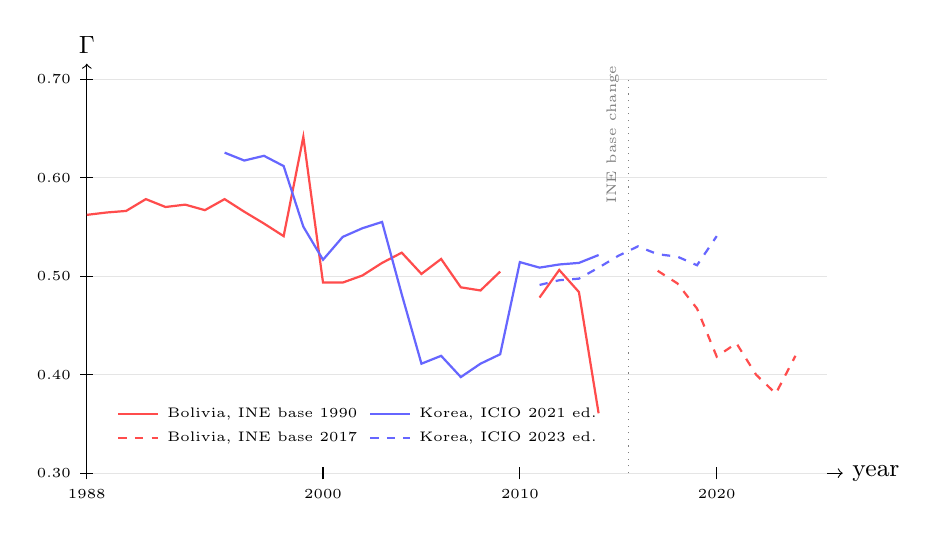
\begin{tikzpicture}[scale=1]
%% x = (year - 1988)/4 cm, y = 12.5 (Gamma - 0.30) cm; coordinates printed by code/ch23.py
\draw[->] (0,0) -- (9.6,0) node[right, font=\small] {year};
\draw[->] (0,0) -- (0,5.2) node[above, font=\small] {$\Gamma$};
\foreach \g/\lab in {0/0.30, 1.25/0.40, 2.5/0.50, 3.75/0.60, 5/0.70} {
  \draw (-0.08,\g) -- (0.08,\g); \node[left, font=\tiny] at (-0.08,\g) {\lab};
  \draw[gray!20] (0.08,\g) -- (9.4,\g);
}
\foreach \x/\yr in {0/1988, 3/2000, 5.5/2010, 8/2020} {
  \draw (\x,-0.08) -- (\x,0.08); \node[below, font=\tiny] at (\x,-0.08) {\yr};
}
%% base change for Bolivia (2014 | 2017)
\draw[gray, dotted] (6.88,0) -- (6.88,5);
\node[font=\tiny, gray, rotate=90, anchor=south] at (6.88,4.3) {INE base change};
%% Bolivia, INE base 1990 (book12)
\draw[red!70, thick] plot coordinates {(0.00,3.28) (0.25,3.31) (0.50,3.33) (0.75,3.48) (1.00,3.38) (1.25,3.41) (1.50,3.34) (1.75,3.48) (2.00,3.32) (2.25,3.17) (2.50,3.01) (2.75,4.27) (3.00,2.42) (3.25,2.42) (3.50,2.51) (3.75,2.67) (4.00,2.80) (4.25,2.53) (4.50,2.72) (4.75,2.36) (5.00,2.32) (5.25,2.56)};
\draw[red!70, thick] plot coordinates {(5.75,2.23) (6.00,2.58) (6.25,2.30) (6.50,0.76)};
%% Bolivia, INE base 2017 (book12)
\draw[red!70, thick, dashed] plot coordinates {(7.25,2.57) (7.50,2.41) (7.75,2.09) (8.00,1.48) (8.25,1.65) (8.50,1.25) (8.75,1.01) (9.00,1.49)};
%% Korea, ICIO 2021 and 2023 editions (book12_isic)
\draw[blue!60, thick] plot coordinates {(1.75,4.07) (2.00,3.97) (2.25,4.03) (2.50,3.90) (2.75,3.13) (3.00,2.71) (3.25,3.00) (3.50,3.11) (3.75,3.19) (4.00,2.27) (4.25,1.39) (4.50,1.49) (4.75,1.22) (5.00,1.39) (5.25,1.51) (5.50,2.68) (5.75,2.61) (6.00,2.65) (6.25,2.67) (6.50,2.77)};
\draw[blue!60, thick, dashed] plot coordinates {(5.75,2.39) (6.00,2.45) (6.25,2.47) (6.50,2.61) (6.75,2.76) (7.00,2.88) (7.25,2.78) (7.50,2.75) (7.75,2.64) (8.00,3.01)};
%% legend
\draw[red!70, thick] (0.4,0.75) -- (0.9,0.75); \node[right, font=\tiny] at (0.9,0.75) {Bolivia, INE base 1990};
\draw[red!70, thick, dashed] (0.4,0.45) -- (0.9,0.45); \node[right, font=\tiny] at (0.9,0.45) {Bolivia, INE base 2017};
\draw[blue!60, thick] (3.6,0.75) -- (4.1,0.75); \node[right, font=\tiny] at (4.1,0.75) {Korea, ICIO 2021 ed.};
\draw[blue!60, thick, dashed] (3.6,0.45) -- (4.1,0.45); \node[right, font=\tiny] at (4.1,0.45) {Korea, ICIO 2023 ed.};
\end{tikzpicture}
\end{center}
\vspace{-0.5em}
\small $\Gamma$ of the 12-sector domestic input-share matrix, by year. Bolivia (red): INE base 1990, 1988--2014 (there is no 2010 table), and base 2017, 2017--2024; the two series are not comparable and are not joined. Korea (blue): OECD ICIO 2021 edition, 1995--2014, and 2023 edition, 2011--2020 (the editions differ by 0.017 in the overlap year 2011). Bolivia is on the book's 12-sector classification and Korea on the ISIC-based one; in 2019 the two classifications give Bolivia 0.467 and 0.475. Both economies' $\Gamma$ fell: Bolivia's from 0.567 (1990) to 0.484 (2013), Korea's from 0.626 (1995) to a trough of 0.397 (2007) and 0.511 in 2019. Over 1995--2019, Korea's ECI rose from 1.10 to 1.81 and Bolivia's fell from $-0.85$ to $-1.30$. Bolivia's 1999 spike and 2014 drop are the break-test flags of Example~\ref{ch23:ex:epochs}. $\sigma_B$ is not plotted: there is no sourced series. Sources: \citet{ine2026sut,oecd2021icio,oecd2023icio,growthlab2026atlas}; author's calculations (\path{data/compute/compute_bolivia_io.py}, \path{data/compute/compute_oecd_io.py}); coordinates from \texttt{code/ch23.py}.
\end{vizpanel}

\begin{keyinsight}
The trajectory panel does not show what the usual story leads one to expect. On a like-for-like 12-sector basis, Bolivia's production network is not a fragmented outlier: its $\Gamma$ (0.475 in 2019, ISIC basis) lies inside the range of the comparators, between the United States (0.463) and Korea (0.511), below Germany (0.544) and Mexico (0.649). And $\Gamma$ fell in both economies: in Bolivia from 0.567 (1990) to 0.484 (2013), in Korea from 0.626 (1995) to 0.511 (2019). Aggregate $\Gamma$ does not separate the two development paths.

What separates them is complexity and where power sits. Korea's ECI rose from 1.10 to 1.81 over 1995--2019, and the Perron vector of its production network concentrated on manufacturing ($G(\boldsymbol{\pi})$ rose from 0.618 to 0.658). That concentration is industrial depth, not fragmentation, and not oppression: in an input-share matrix, a high $\pi$ marks a hub that many sectors buy from. Bolivia's ECI fell from $-0.85$ to $-1.30$. Its enclave shows up not in $\Gamma$ but in $\boldsymbol{\pi}$ and export orientation: in 2019 hydrocarbons had a Perron weight of 0.039 and exported 70\% of their output (Chapter~20).

Nor did distributional progress wait for $\Gamma$. Bolivia grew at 4.0\% a year over 1990--2019, its Gini fell from 0.600 (2005) to 0.426 (2019), and extreme poverty from 38.2\% to 15.2\% (2005--2018), while $\Gamma$ drifted down and ECI fell. On this chapter's reading, the gains came mostly through transfers and labour-market tightening within the existing structure ($\Delta\boldsymbol{\omega}$) rather than through $\Delta W$. Whether they can be sustained without structural change is the open question of Chapter~26. That they happened at all is evidence against any claim that equity gains \emph{require} rising $\Gamma$ or positive ECI.

Korea's transformation (land reform, mass education, export discipline, industrial policy) began decades before 1995, and its $\Gamma$ in those decades is not measured here: pre-1995 Korean tables were not available. Whatever that path was, Korea entered 1995 with $\Gamma$ above 0.6, so its development cannot be read as a rise in aggregate integration over the years the data cover.

A structural report card needs several coordinates. $\Gamma$ alone grades Korea and Bolivia alike.
\end{keyinsight}


%% =====================================================================
\section{Speed of Structural Change}
\label{ch23:sec:speed}
%% =====================================================================

\begin{definition}[Structural Velocity]\label{ch23:def:velocity}
The \textbf{structural velocity} is the rate of change of the spectral gap:
\begin{equation}\label{ch23:eq:velocity}
v_\Gamma(t) = \frac{\Gamma_{t+1} - \Gamma_t}{\Delta t}.
\end{equation}
The \textbf{structural acceleration} is $a_\Gamma(t) = v_\Gamma(t+1) - v_\Gamma(t)$.
\end{definition}

\begin{example}[Structural Velocities, Selected Countries]\label{ch23:ex:velocities}
Endpoint velocities $v_\Gamma = (\Gamma_T - \Gamma_{t_0})/(T - t_0)$, per decade, computed within each data vintage:
\begin{center}
\begin{tabular}{lcc}
\toprule
Country & 1995--2014 (ICIO 2021) & 2011--2020 (ICIO 2023) \\
\midrule
South Korea & $-0.055$ & $+0.055$ \\
Chile & $+0.091$ & $+0.107$ \\
Argentina & $+0.037$ & $-0.050$ \\
Germany & $-0.002$ & $+0.043$ \\
United States & $-0.010$ & $-0.016$ \\
China & n/a & $-0.038$ \\
\midrule
 & 1990--2013 (INE base 1990) & 2017--2024 (INE base 2017) \\
Bolivia & $-0.036$ & $-0.12$ \\
\bottomrule
\end{tabular}
\end{center}
\par{\footnotesize Source: OECD ICIO, 2021 and 2023 editions \citep{oecd2021icio,oecd2023icio}, ISIC-based 12 sectors; INE input--output matrices and supply-use tables \citep{ine2026sut}, book's 12 sectors; domestic flows, input shares. Author's calculations (\path{data/compute/compute_velocity.py}, \path{data/processed/gamma_velocity.csv}). China is split into two blocks in the 2021 edition and could not be extracted for 1995--2010. Venezuela is not a separate economy in ICIO. OLS slopes for Bolivia: $-0.046$ and $-0.16$.\par}

Three things stand out. First, the signs flip. Korea's $\Gamma$ fell at 0.055 per decade over 1995--2014 and rose at the same speed over 2011--2020; Argentina's did the reverse. At the 12-sector level, $v_\Gamma$ is not a stable property of a country, and over a decade it is of the same order as the year-to-year noise in $\Gamma_t$. Second, $v_\Gamma$ does not track development. The fastest ``integrator'' in the table is Chile, whose ECI barely moved (about 0.1 in 1995, $-0.06$ in 2019). Among the most negative entries are Korea over 1995--2014, when its ECI rose from 1.10 to 1.70, and China, whose ECI also rose (1.15 in 2010, 1.30 in 2019). Third, Bolivia's $\Gamma$ fell in both of its series ($-0.036$ per decade over 1990--2013; $-0.12$ over 2017--2024, a window that includes the pandemic). There is no ``distance to Korea'' to close in $\Gamma$: on the cross-country basis, Bolivia's 2019 value (0.475) is within 0.04 of Korea's (0.511).
\end{example}

\begin{remark}[What Determines Structural Velocity?]\label{ch23:prop:velocity_determinants}
The co-evolutionary dynamics of Chapter~13 suggest that structural velocity depends on the following (a list of channels, not a derived result):
\begin{enumerate}
\item \textbf{Cross-block surplus} $s_{\text{cross}}$: higher surplus makes new cross-block edges profitable. Industrial policy that creates cross-block linkages increases $v_\Gamma$.
\item \textbf{Edge destruction rate} $\delta_{\text{cross}}$: crises, policy reversals, and political instability destroy cross-block edges, reducing $v_\Gamma$ or making it negative.
\item \textbf{Proximity bias} $p_1$: strong path dependence (high $p_1$) slows diversification into structurally distant activities, capping $v_\Gamma$.
\item \textbf{Formation velocity}: the speed at which preferences adjust ($1 - \rho$). Fast preference adjustment ($\rho$ small) allows rapid norm change, which supports structural change. Slow adjustment ($\rho$ large; the book's illustrative Bolivian value is $\rho \approx 0.85$) means preferences lag behind structure, creating resistance to change.
\end{enumerate}
\end{remark}


%% =====================================================================
\section{Distinguishing Structural Change from Cyclical Fluctuation}
\label{ch23:sec:distinguish}
%% =====================================================================

\begin{definition}[Structural-Cyclical Decomposition]\label{ch23:def:decomposition}
Any change in the Perron eigenvector can be written as
\begin{equation}\label{ch23:eq:SC_decomp}
\Delta\pi_{i,t} = \underbrace{\Delta\pi_{i,t}^S}_{\text{structural}} + \underbrace{\Delta\pi_{i,t}^C}_{\text{cyclical}},
\end{equation}
where:
\begin{enumerate}
\item The \textbf{structural component} $\Delta\pi^S$ is the part of the change that \emph{persists}: the change in the trend of $W_t$, whatever its origin (new edges, destroyed edges, or a lasting reweighting such as a new fiscal regime).
\item The \textbf{cyclical component} $\Delta\pi^C$ is the part that \emph{reverses}: transitory deviations of $W_t$ from its trend due to price fluctuations, demand shocks, or temporary policy.
\end{enumerate}
The criterion is persistence, not the type of break (Definition~\ref{ch23:prop:break_types}). Identification: filter each series $\pi_{i,t}$ separately (HP or band-pass, Appendix~\ref{ch23:app:decomposition}); its trend is $\pi^S_{i,t}$ and the residual is $\pi^C_{i,t}$. The same filter applied to $\Gamma_t$ gives the structural and cyclical parts of integration. This is a definition, not a theorem: the split depends on the filter and its smoothing parameter.
\end{definition}

\begin{example}[Bolivia: The Gas Boom in $\boldsymbol{\pi}$, 2003--2024]\label{ch23:ex:decomposition}
During the gas boom, the hydrocarbons sector's Perron weight in the domestic $W^P$ rose from 0.047 (2003) to 0.085 (2013), and to 0.117 in 2014, a year whose $\Gamma$ is an outlier (Example~\ref{ch23:ex:epochs}). On base 2017 it was 0.045 in 2017, 0.039 in 2019 and 0.021 in 2024. The sector's share of gross value added followed the same arc: 3.5\% (2000), 7.9\% (2006) and 10.0\% (2013) on base 1990; 6.3\% (2017) and 3.3\% (2024) on base 2017.
\par{\footnotesize Source: INE input--output matrices (base 1990) and supply-use tables (base 2017), 12 sectors, domestic flows, input shares \citep{ine2026sut}; author's calculations (\path{data/compute/compute_bolivia_io.py}, \path{data/compute/compute_bolivia_facts.py}).\par}

The change of base blocks the decomposition that Definition~\ref{ch23:def:decomposition} calls for. No single series runs from before the boom to after it, so the 2019 level cannot be compared with the 2003 level, and a filter run across the break would read the change of base as structural. Within each base the pattern is clear. The rise in $\pi_{\text{gas}}$ tracked the price and volume boom, and on the new base the weight kept falling as production declined. The data show no sign of a persistent increase in the sector's place in the domestic network. Whatever the nationalization changed permanently, it was the fiscal capture of rents (Epoch~3), which $W^P$ does not record.

Note also the scale. Even at its peak, $\pi_{\text{gas}}$ was never far above the uniform share $1/N \approx 0.09$: the sector was never a hub of the domestic network. Its weight lay in exports and fiscal revenue, not in domestic linkages. An analysis that counted Bolivia's boom as ``structural transformation'' was reading a cyclical rise in a peripheral sector's weight.
\end{example}

\begin{prebisch}[Commodity booms as cyclical mirages]
Latin American economic history is a sequence of commodity booms mistaken for structural change. Guano in Peru (1840--1870), nitrate in Chile (1880--1920), coffee in Brazil (1890--1930), oil in Venezuela (1920--2015), gas in Bolivia (2003--2014). Each boom raised incomes, reduced poverty, and generated optimism about ``transformation.'' Each bust revealed that the production structure had not changed: the economy remained an enclave connected to the world through a single commodity edge. The enclave is not a matter of aggregate $\Gamma$, which in Bolivia is in the range of industrial economies. It is a matter of where the commodity sector sits: at the periphery of the domestic network (a small $\pi$), exporting most of its output, buying few domestic inputs, and paying a small share of its value added as wages.

The structural-cyclical decomposition is the instrument that detects the mirage. During the boom: $\Delta\pi^C$ is large (the commodity sector's weight inflates). After the bust: $\Delta\pi^C$ reverses. The structural component $\Delta\pi^S$ is what remains --- and it is typically near zero for commodity booms, because commodity booms do not create cross-block domestic linkages.

The exception: commodity booms CAN produce structural change if the revenue is invested in the operators of Chapter~15 (information, education, infrastructure, industrial policy). Norway is the canonical example, though not through its oil fund: the Government Pension Fund Global invests only abroad, precisely to keep oil revenue out of the domestic economy. Norway's structural change came from building domestic supplier, engineering and technology capabilities around the petroleum sector. Neither aggregate used in this chapter shows it, however. On the 12-sector ICIO basis Norway's $\Gamma$ fell from 0.644 in 1995 to 0.313 in 2014, as the economy reorganized around petroleum and its supply industries, and its ECI fell from 1.24 to 1.01 (\citealp{oecd2021icio,growthlab2026atlas}; \path{data/processed/gamma_velocity.csv}, \path{eci_facts.csv}). If the petroleum cluster is structural change, it is visible only at a finer grain: in the domestic input intensity of the petroleum sector and the exports of its suppliers. That is where a test would have to look. Bolivia's gas revenue went largely into transfers ($\Delta\boldsymbol{\omega}$): poverty fell sharply, $\Gamma$ drifted down, and ECI fell.
\end{prebisch}


%% =====================================================================
\section{The Structural Change Index}
\label{ch23:sec:index}
%% =====================================================================

\begin{definition}[Structural Change Index (SCI)]\label{ch23:def:SCI}
The \textbf{Structural Change Index} summarizes the entire trajectory in a single number:
\begin{equation}\label{ch23:eq:SCI}
\text{SCI}(t_0, T) = \frac{\Gamma_T - \Gamma_{t_0}}{\Gamma^{\text{ref}} - \Gamma_{t_0}},
\end{equation}
where $\Gamma^{\text{ref}} > \Gamma_{t_0}$ is a reference level of integration chosen by the analyst (here $\Gamma^{\text{ref}} = 0.50$, a round number near Germany's 0.544 in 2019 on the 12-sector ICIO basis). It is a normalization, not the estimated threshold $\Gamma^*$ of Chapter~26. SCI is the fraction of the distance to the reference closed over the period: it equals 0 if nothing changed and 1 if the reference was reached, is negative when integration fell (the United States in Example~\ref{ch23:ex:SCI}), can exceed 1 on overshoot, and is undefined when $\Gamma_{t_0} \ge \Gamma^{\text{ref}}$.
\end{definition}

\begin{example}[SCI for Selected Countries]\label{ch23:ex:SCI}
Using $\Gamma^{\text{ref}} = 0.50$ and the 1995--2014 window of the ICIO 2021 edition (Bolivia: INE base 1990, 1990--2013):
\begin{center}
\begin{tabular}{lcccc}
\toprule
Country & $\Gamma_{t_0}$ & $\Gamma_T$ & Period & SCI \\
\midrule
Chile & 0.467 & 0.640 & 1995--2014 & $5.30$ \\
Argentina & 0.407 & 0.476 & 1995--2014 & $0.75$ \\
United States & 0.475 & 0.457 & 1995--2014 & $-0.72$ \\
South Korea & 0.626 & 0.522 & 1995--2014 & undefined \\
Germany & 0.554 & 0.549 & 1995--2014 & undefined \\
Bolivia & 0.567 & 0.484 & 1990--2013 & undefined \\
\bottomrule
\end{tabular}
\end{center}
\par{\footnotesize Source: as for Example~\ref{ch23:ex:velocities}. The SCI is recomputed by \texttt{code/ch23.py} from the file \path{data/processed/gamma_velocity.csv}.\par}

With the real trajectories the index is mostly undefined. Korea, Germany and Bolivia all start above $\Gamma^{\text{ref}}$, so on this basis they have ``no gap to close''. Where the index is defined, the denominator dominates it: Chile's 5.30 comes from a gap of only 0.033, overshot fivefold. The SCI presumes that development means moving $\Gamma$ from far below a reference to the reference. At the 12-sector level the data supply no such gradient: in 2019, $\Gamma$ for economies as different as Bolivia, Korea, Germany and the United States lies between 0.46 and 0.54. An index of this form is informative only for an indicator with a clear developmental gradient and starting points far from the reference. On this evidence that points to ECI, or to finer-grained network measures, rather than to aggregate $\Gamma$.
\end{example}


%% =====================================================================
\section{Summary}
\label{ch23:sec:summary}
%% =====================================================================

\begin{enumerate}
\item The \textbf{structural trajectory} $\{(\Gamma_t, \sigma_{B,t}, G(\boldsymbol{\pi}_t), N_{\text{eff},t}, \text{ECI}_t)\}$ is the time series of structural health. In the data (INE base 1990 and base 2017, kept separate; OECD ICIO 1995--2019), $\Gamma$ \emph{fell} in both Bolivia (0.567 in 1990, 0.484 in 2013) and Korea (0.626 in 1995, 0.511 in 2019). Complexity separates them: Korea's ECI rose from 1.10 to 1.81, Bolivia's fell from $-0.85$ to $-1.30$.

\item \textbf{Structural breaks} are detectable as discontinuities in $\Gamma_t$, once bootstrap error bands are respected. Per-period $\Gamma_t$ does not control the product $W_t\cdots W_s$: the Dobrushin coefficient $\tau_1$ and the realized-product gap do, and the absolute probability sequence is the time-varying power vector. Bolivia's series shows no break that matches a policy event; the flagged years (1999--2000, 2014) look like effects of how the tables were built.

\item \textbf{Structural velocity} $v_\Gamma$ measures the speed of integration. Bolivia: $-0.036$ per decade (1990--2013) and $-0.12$ (2017--2024). Korea: $-0.055$ (1995--2014) and $+0.055$ (2011--2020). At the 12-sector level, velocities flip sign between windows and do not track development.

\item The \textbf{structural-cyclical decomposition} (a definition, based on persistence) separates permanent changes in $W$ from temporary price effects. Commodity booms are cyclical: $\Delta\pi^C$ reverses after the boom. Bolivia's $\pi_{\text{gas}}$ rose from 0.047 (2003) to 0.085 (2013) and, on the new base, fell to 0.021 (2024); the change of base prevents a clean decomposition. The sector stayed peripheral in the domestic network throughout.

\item The \textbf{Structural Change Index} (SCI): fraction of the distance to a reference $\Gamma$ closed (negative if integration falls). With $\Gamma^{\text{ref}} = 0.50$ it is undefined for Korea, Germany and Bolivia, which start above the reference: aggregate $\Gamma$ supplies no developmental gradient for it to measure.
\end{enumerate}


%% =====================================================================
\section{Exercises}
\label{ch23:sec:exercises}
%% =====================================================================

\begin{enumerate}[label=\textbf{23.\arabic*}, leftmargin=3em]

\item \textbf{Bolivia's trajectory.} Using INE's input--output matrices (base 1990) and supply-use tables (base 2017), and EH microdata: construct Bolivia's structural trajectory for 2000--2019, keeping the two bases separate. Plot $\Gamma_t$ against $G(\boldsymbol{\pi}_t)$ and, if you can compute it from the EH, against $\sigma_{B,t}$. Which coordinates move? Repeat with sales shares and with the diagonal removed: does the direction of change survive?

\item \textbf{Structural break detection.} Compute $\Delta\Gamma_t$ for each year. Apply the break detection criterion with $k = 2$, and a bootstrap band (Remark~\ref{ch23:rem:conditioning}). Are there any structural breaks? At what years? Do they correspond to policy events? Compute $\tau_1(W_t)$ and the realized-product gap $\Gamma^{(5)}_t$ as well: do they tell the same story as $\Gamma_t$?

\item \textbf{Structural velocity.} Compute $v_\Gamma$ for Bolivia (INE), Chile and Peru (OECD ICIO), by endpoints and by OLS. Does each country's velocity keep its sign across the 1995--2014 and 2011--2020 windows? Compare it with each country's change in ECI over the same years. What does the comparison say about $v_\Gamma$ as a measure of development?

\item \textbf{Structural-cyclical decomposition.} For Bolivia, decompose $\pi_{\text{gas},t}$ into structural and cyclical components with an HP filter, on the base-1990 series only (1988--2014). How much of the 2003--2013 rise was structural? How sensitive is the answer to $\lambda$, and to dropping the 2014 outlier? Why must the base-2017 years not be appended to the series?

\item \textbf{Commodity boom counterfactual.} Suppose Bolivia had invested 30\% of gas revenue in cross-block operators (infrastructure connecting gas to traditional sector, technical education for rural workers). Simulate the effect on the hydrocarbons sector's domestic input intensity (0.225 per unit of output in 2019), on its Perron weight, and on $\Gamma$. Which of the three indicators would detect the change, and why might $\Gamma$ not?

\item \textbf{SCI computation.} For the Latin American countries covered by the OECD Inter-Country Input-Output tables, compute $\Gamma$ of the row-normalized domestic input-share matrix $W^P = D^{-1}A$ for the first and last available years, using the same sector classification for every country. Compute SCI with $\Gamma^{\text{ref}} = 0.50$ and rank the countries. For how many is it undefined? Now rank them by the change in ECI. Why is ECI \emph{not} a proxy for $\Gamma$? (Hint: ECI is computed from the country--product export matrix and is standardized across countries each year.)

\item \textbf{Trajectory projection.} Bolivia's ECI changed by $-0.44$ over 1995--2019 and by $+0.20$ over 2019--2024; Korea's rose by $+0.70$ over 1995--2019 (\path{data/processed/eci_epochs_bolivia.csv}, \path{eci_facts.csv}). Project Bolivia's ECI for 2025--2060 under three scenarios: (a) the 1995--2019 trend, (b) the 2019--2024 trend, (c) Korea's 1995--2019 pace. Plot all three. When, if ever, does each reach $\text{ECI} = 0$? ECI is standardized across countries each year: what does a ``trend'' in it mean?
\end{enumerate}


%% =====================================================================
\newpage
\section*{Mathematical Appendices}
\addcontentsline{toc}{section}{Mathematical Appendices}
%% =====================================================================


\subsection*{Appendix 23A: The RAS Method for I-O Table Updating}
\addcontentsline{toc}{subsection}{Appendix 23A: RAS Method}
\label{ch23:app:RAS}

\paragraph{Problem.} Given a benchmark I-O coefficient matrix $A_0$ and new row totals $\mathbf{r}$ and column totals $\mathbf{c}$, find the updated matrix $A^*$ that matches the new margins while staying ``close'' to $A_0$.

\paragraph{Algorithm.} The RAS (or biproportional) method alternates row and column scaling:
\begin{enumerate}
\item Initialize $A^{(0)} = A_0$.
\item Scale rows: $A^{(2k+1)}_{ij} = A^{(2k)}_{ij} \cdot r_i / \sum_j A^{(2k)}_{ij}$.
\item Scale columns: $A^{(2k+2)}_{ij} = A^{(2k+1)}_{ij} \cdot c_j / \sum_i A^{(2k+1)}_{ij}$.
\item Repeat until convergence.
\end{enumerate}

When it exists, the RAS solution minimizes the KL-divergence
\[
\textstyle\sum_{ij} A^*_{ij}\ln(A^*_{ij}/A_{0,ij})
\]
subject to the margin constraints. It preserves zeros (if $A_{0,ij} = 0$ then $A^*_{ij} = 0$) and the block structure of $A_0$. Existence requires $\sum_i r_i = \sum_j c_j$ and margins compatible with the zero pattern of $A_0$ \citep{bacharach1970biproportional}; in practice the iteration is applied to intermediate transactions, whose margins are intermediate sales and purchases, and the result is row-normalized afterwards to obtain $W^P_t$.

\paragraph{Structural interpretation.} RAS updating assumes the block structure of $W^P$ is unchanged between benchmarks --- only the relative sizes of sectors change. This is conservative: it cannot detect edge creation or destruction between benchmark I-O tables. Between benchmarks, $\Gamma_t$ moves only through the margins. Real structural change therefore shows up as a jump \emph{at the next benchmark year}, which then bundles several years of accumulated change; do not read the jump as a one-year break.


\subsection*{Appendix 23B: Structural vs.\ Cyclical Decomposition}
\addcontentsline{toc}{subsection}{Appendix 23B: Structural-Cyclical Decomposition}
\label{ch23:app:decomposition}

\paragraph{HP filter.} The Hodrick-Prescott filter decomposes $\Gamma_t = \Gamma_t^S + \Gamma_t^C$ by minimizing $\sum_t (\Gamma_t - \Gamma_t^S)^2 + \lambda\sum_t [(\Gamma_{t+1}^S - \Gamma_t^S) - (\Gamma_t^S - \Gamma_{t-1}^S)]^2$. The smoothing parameter $\lambda$ controls the trade-off between fit and smoothness. For annual data: $\lambda = 6.25$ \citep{ravn2002adjusting} or $\lambda = 100$ (traditional). These choices matter: the gain-$\tfrac12$ cutoff period of the annual HP filter is about 10 years for $\lambda = 6.25$, 20 years for $\lambda = 100$, 28 years for $\lambda = 400$ and 40 years for $\lambda = 1600$ (\texttt{code/ch23.py}). To separate a 10--20 year cycle from structural trends use $\lambda \approx 6.25$--$100$; $\lambda = 400$--$1600$ treats everything shorter than 28--40 years as cyclical.

\paragraph{Band-pass filter.} The Baxter-King or Christiano-Fitzgerald filter isolates fluctuations at specific frequencies. Structural change: periods $> 20$ years. Business cycle: 2--8 years. The band-pass filter cleanly separates the two.

\paragraph{Structural breaks.} The HP and band-pass filters assume smooth trends. For detecting abrupt structural breaks (nationalization, crisis, regime change): use the \citet{bai1998estimating} multiple structural break test applied to $\Gamma_t$. The null hypothesis is no break; the alternative is one or more breaks at unknown dates.


%% =====================================================================
\subsection*{Structuralist Case Study: CEPAL's Structural Change Program}
\addcontentsline{toc}{subsection}{Structuralist Case Study: CEPAL (2012)}
%% =====================================================================

\citeauthor{cepal2012structural}'s (\citeyear{cepal2012structural}) report \textit{Structural Change for Equality: An Integrated Approach to Development} represents the institutional synthesis of the structuralist tradition's diagnosis and prescription. Published 63 years after Prebisch's \citeyear{prebisch1949desarrollo} manifesto, it argues that Latin America's central challenge remains structural: the region has achieved macroeconomic stability and poverty reduction but has not changed its production structure.

The report maps onto this chapter's framework precisely.

\textbf{Part 1: Structural change is slow.} CEPAL documents that Latin America's export composition changed little over 1990--2010: the region remained specialized in natural resources and low-technology manufactures. In this chapter's terms, the complexity trajectory was flat or falling: Chile's ECI was about 0.1 in 1995 and $-0.06$ in 2019, and Bolivia's fell from $-0.85$ to $-1.30$. The $\Gamma$ velocities are small and of mixed sign (1995--2014, per decade: Chile $+0.091$, Argentina $+0.037$, Brazil $+0.020$, Colombia $-0.036$, Peru $-0.060$; Example~\ref{ch23:ex:velocities}), and, as for Korea, they do not track development.

\textbf{Part 2: Redistribution without structural change is unsustainable.} CEPAL notes that the region's poverty reduction (2000--2012) was driven by commodity booms and fiscal transfers, not by structural transformation. In this chapter's terms: $\Delta\boldsymbol{\omega} \gg \Delta W$. The improvement is cyclical ($\Delta\pi^C > 0$ during the boom) not structural ($\Delta\pi^S \approx 0$). When the commodity cycle reversed (post-2014), poverty stagnated and in some countries reversed.

\textbf{Part 3: The prescription is ``change for equality.''} CEPAL argues for industrial policy, technological upgrading, and institutional reform --- the operators of Chapter~15, stated in institutional language rather than matrix notation. The report's title states a claim: structural change ($\Delta\Gamma > 0$) is necessary for sustained equality ($\sigma_B \downarrow$). In this book that claim is not a theorem; it is the testable conjecture of Chapter~26 (Conjecture~\ref{ch26:conj:growth_equity}). Bolivia's record is evidence against it in its $\Gamma$ form: between 2005 and 2019 the Gini fell from 0.600 to 0.426 while $\Gamma$ drifted down and ECI fell. The claim survives only as one about \emph{sustaining} equity gains, not achieving them.

\begin{center}
\begin{tabularx}{\textwidth}{LLL}
\toprule
\textbf{\citet{cepal2012structural}} & \textbf{This chapter} & \textbf{Cross-reference} \\
\midrule
Structural change is slow & ECI flat or falling; $v_\Gamma$ of mixed sign & Ex.~\ref{ch23:ex:velocities} \\
Redistribution without structural change & $\Delta\boldsymbol{\omega} \gg \Delta W$ & Sec.~\ref{ch23:sec:bolivia}, Epoch 4 \\
Commodity boom as mirage & $\Delta\pi^C$ reverses & Prebisch Connection \\
Change for equality & $\Delta\Gamma > 0$ needed? Not in Bolivia 2005--19 & Conjecture (Ch.~26) \\
Policy: industrial upgrading & Operators from Ch.~15 & Ch.~15 \\
SCI as metric & Fraction of gap closed & Def.~\ref{ch23:def:SCI} \\
\bottomrule
\end{tabularx}
\end{center}

CEPAL wrote in the language of institutions and policy. This chapter translates into eigenvalues and trajectories. The message is largely the same: Latin America has been redistributing within a structure that, measured by what it can produce and export, has not changed. The data add a warning CEPAL did not need to make. At this level of aggregation, the integration of the input--output network is not where the missing structural change shows up: Bolivia's $\Gamma$ is like Korea's, and both fell.


%% =====================================================================
\subsection*{Further Reading}
\addcontentsline{toc}{subsection}{Further Reading}
%% =====================================================================

\textbf{Structural change measurement:} \citet{cepal2012structural}, \textit{Structural Change for Equality}. \citet{mcmillan2014globalization}, ``Globalization, Structural Change, and Productivity Growth.'' \citet{devries2012deconstructing}, ``Deconstructing the BRICs.''

\textbf{I-O table updating:} \citet{miller2009inputoutput}, \textit{Input-Output Analysis: Foundations and Extensions}, Chapter~8 (RAS and cross-entropy methods). \citet{temursho2018entropy}, ``Entropy-Based Benchmarking Methods.''

\textbf{Structural breaks:} \citet{bai1998estimating}, ``Estimating and Testing Linear Models with Multiple Structural Changes.'' For application to development: \citet{pritchett2000understanding}, ``Understanding Patterns of Economic Growth.''

\textbf{Data used in this chapter:} INE input--output matrices and supply-use tables \citep{ine2026sut}; OECD ICIO \citep{oecd2021icio,oecd2023icio}; Growth Lab complexity data \citep{growthlab2026atlas}; World Development Indicators \citep{worldbank2026wdi}. Scripts and processed files are in \path{data/}.

\textbf{Bolivia's economic history:} \citet{morales1990bolivias}, ``Bolivia's Economic Crisis.'' \citet{weisbrot2009bolivia}, ``Bolivia: The Economy During the Morales Administration.'' Andersen et al.\ (2020), ``Bolivia's Twenty-First Century Commodity Boom,'' INESAD Working Paper.

\end{document}
